\documentclass[10pt,a4paper]{report}

\usepackage[utf8]{inputenc}
\usepackage[T1]{fontenc}
\usepackage[top=2cm,bottom=2cm]{geometry}
\usepackage{todo}
\usepackage{amssymb}
\usepackage{graphicx,tabularx}
\usepackage{amsmath,amsfonts}%
\usepackage{amsthm}
\usepackage{nicefrac}
\usepackage{xcolor}
\usepackage{bm}%
\usepackage{psfrag}%
\usepackage{pict2e}
% \usepackage{mdframed,verbatim}
\usepackage[tikz]{bclogo}
\usepackage{epstopdf}
\usepackage[colorlinks=true, pdfstartview=FitV, linkcolor=blue,
            citecolor=blue, urlcolor=blue]{hyperref}
\usepackage{tikz}
\usetikzlibrary{decorations.pathmorphing,patterns}
\usepackage[europeanresistors]{circuitikz}
\usepackage{pgfplots}
\newif\ifsolutions
\solutionstrue
% \solutionsfalse
\usepackage{commands_od}

\newcommand\dd{\mathrm{d}}

% ------------------- Title and Author -----------------------------

\begin{document}




\begin{center}
{\Large Projet Matélec }
 \begin{tabularx}{\linewidth}{c}
\hline
\end{tabularx}
\end{center}
\begin{center}
{\Large \textbf{Examen sur les outils mathématiques}\\}
\end{center}
 \begin{tabularx}{\linewidth}{c}
\hline
\end{tabularx}
\setcounter{chapter}{1}

\bigskip

\tb{Modalités}
\begin{itemize}
	\item Ce Contrôle Continu dure 1 heure et 30 minutes et comporte 3 exercices indépendants.
	\item Le \textbf{formulaire} est autorisé, tout \textbf{autre document est interdit}.
	\item La \textbf{calculatrice est interdite}.
\end{itemize}

\bigskip

\bexo

Trouver les racines des polynômes suivants :

\begin{enumerate}
	\item $3x^3 - 3x^2$
	\item $x^2 + 2x + 4$
\end{enumerate}


\bigskip


\eexo

\bexo
On considère un système constitué d'une masse $m$ reliée à un bâti rigide à l'aide d'un ressort $k$. Cette masse est également soumise à une force extérieure constante égale à $1$. Le déplacement $x(t)$ de la masse obéit à l'équation suivante
\begin{equation}
	mx''(t)+kx(t)=t.
\end{equation}
On considère les conditions initiales 
\begin{equation}
	x(0)=0,\, x'(0)=0.
\end{equation}
\begin{itemize}
	\item Etant donné le second membre, sous quelle forme chercher la solution particulière de cette équation différentielle? 
	\item Donner une solution particulière.
	\item Donner l'expression du déplacement $x(t)$.
	\item Quel est l'analogue électrique ce système ?
\end{itemize}



\eexo


\newpage
\bexo

On considère un circuit électrique composé d'une bobine d'inductance $L$ et d'une
résistance $R$ en série avec un générateur de tension délivrant une tension continue $E$.

\begin{center}
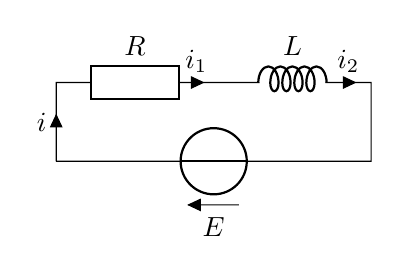
\begin{tikzpicture}[scale=1]
	\draw (0,0) to[short, i=$i$] (0,1) to[R=$R$, i=$i_1$] (2,1) to[L=$L$, i=$i_2$] (4,1) to[short] (4,0) to[V=$E$] (0,0);
\end{tikzpicture}
\end{center}

\begin{enumerate}
	\item Rappeler les deux lois fondamentales d'électricité s'appliquant dans le circuit.
	\item Montrer que l'équation différentielle régissant l'évolution du courant $i$ dans le
		circuit est \[L\frac{\dd i(t)}{\dd t} + Ri(t) = E\]
	\item En considérant une analogie courant-vitesse, établir le lien entre le système
		électrique et la chute d'une masse ($m$) en fluide visqueux (constante de frottement
		$c$). Rappeler l'équation différentielle pour le système mécanique et établir la
		correspondance entre les quantités des deux domaines.
	\item Déduire des équations différentielles les constantes de temps $\tau$ mécaniques et
		électriques telles que: $x(t) = \alpha e^{\nicefrac{t}{\tau}}$ (avec $\alpha$ une constante).
	\item On considère que la masse du système mécanique commence sa chute sans vitesse
		initiale. Transcrire cette condition initiale dans le domaine électrique.
	\item Résoudre l'équation différentielle dans le domaine électrique.
	\item Tracer l'allure de l'intensité en fonction du temps.
\end{enumerate}

À toutes fins utiles, on rappelle les lois de comportement suivantes (convention
récepteur) :

\begin{equation*}
	q(t) = CU_C(t) ~~,~~ i_C(t) = \frac{\dd q(t)}{\dd t} ~~,~~ U_L(t) = L\frac{\dd i_L(t)}{\dd t} ~~,~~ U_R(t)
	= Ri_R(t)
\end{equation*}

\bigskip

\eexo



\end{document}
\end

